\documentclass[12pt]{article}
\usepackage[letterpaper, total={6in, 8in}]{geometry}
\setlength{\oddsidemargin}{0in}
\setlength{\evensidemargin}{0in}
\setlength{\textwidth}{6.5in}
\setlength{\parindent}{0in}
\setlength{\parskip}{\baselineskip}

\usepackage{amsmath,amsfonts,amssymb}
\usepackage{subfigure}
\usepackage{sectsty}
\usepackage{multirow}
\usepackage{makecell}
\usepackage{float}
\usepackage[utf8x]{inputenc}
\usepackage[pdftex]{graphicx}
\usepackage[toc,page]{appendix}
\usepackage{enumitem}
\usepackage{indentfirst}
\usepackage{scrextend}
\usepackage{caption}
\usepackage{hyperref}
\usepackage{adjustbox}

\usepackage{listings}
\usepackage{color} %red, green, blue, yellow, cyan, magenta, black, white
\definecolor{mygreen}{RGB}{28,172,0} % color values Red, Green, Blue
\definecolor{mylilas}{RGB}{170,55,241}

\DeclareFixedFont{\ttb}{T1}{txtt}{bx}{n}{10} % for bold
\DeclareFixedFont{\ttm}{T1}{txtt}{m}{n}{10}  % for normal

\usepackage{color}
\definecolor{deepblue}{rgb}{0,0,0.5}
\definecolor{deepred}{rgb}{0.6,0,0}
\definecolor{deepgreen}{rgb}{0,0.5,0}

\usepackage{sectsty}

\sectionfont{\fontsize{14}{15}\selectfont}
\subsectionfont{\fontsize{12}{15}\selectfont}

\usepackage{listings}
\lstset{language=Matlab,%
	%basicstyle=\color{red},
	breaklines=true,%
	morekeywords={matlab2tikz},
	keywordstyle=\color{blue},%
	morekeywords=[2]{1}, keywordstyle=[2]{\color{black}},
	identifierstyle=\color{black},%
	stringstyle=\color{mylilas},
	commentstyle=\color{mygreen},%
	showstringspaces=false,%without this there will be a symbol in the places where there is a space
	numbers=left,%
	numberstyle={\tiny \color{black}},% size of the numbers
	numbersep=9pt, % this defines how far the numbers are from the text
	emph=[1]{for,end,break},emphstyle=[1]\color{red}, %some words to emphasise
	%emph=[2]{word1,word2}, emphstyle=[2]{style},    
}


% Python style for highlighting
\newcommand\pythonstyle{\lstset{
		language=Python,
		basicstyle=\ttm,
		otherkeywords={self},             % Add keywords here
		keywordstyle=\ttb\color{deepblue},
		emph={MyClass,__init__},          % Custom highlighting
		emphstyle=\ttb\color{deepred},    % Custom highlighting style
		stringstyle=\color{deepgreen},
		frame=tb,                         % Any extra options here
		showstringspaces=false            % 
}}


% Python environment
\lstnewenvironment{python}[1][]
{
	\pythonstyle
	\lstset{#1}
}
{}

% Python for external files
\newcommand\pythonexternal[2][]{{
		\pythonstyle
		\lstinputlisting[#1]{#2}}}

% Python for inline
\newcommand\pythoninline[1]{{\pythonstyle\lstinline!#1!}}

\begin{document}
\hfill Sam Feig $|$ Vladimir Zhdanov \\
\textbf{H5 Report}\hfill CSCI 4831/5722 \\
\rule{\textwidth}{.75pt}

\section{Methods}
\subsection{Color}
	Color segmentation is very effective as it enables the differentiation of objects based on the fact that most objects are not the same as the background of the image they are in front of. This segmentation strategy works very well when objects are well defined have have distinct color differences/edges between them. 
	
	Color segmentation works less well when objects are camouflaged in with the background or have similar colors to other objects or the background of the image.
	
\subsection{Position}
	Adding position segmentation stems from the idea that pixels that are close together are likely to come from the same object and so should be grouped together. This segmentation works well on objects that have clear boundaries but might have more similar colors that color segmentation alone would struggle with.
	
	Position segmentation does not work well when objects that should be clustered together are not near each other in the image, like when an object is obscured by another and so gets split into multiple parts in around the object that is in front of it.
	
\subsection{Edges}
	Adding edge segmentation enables the detection of outlines of objects that can be used to bound segmentation as most segmentation should occur near or on the edge of an object in the image. This works well when there are clear, sharp edges in an image that can be calculated.
	
	Edge segmentation will struggle when it is faced with blurred/smoothed images, or things without clear edges in them as the binary map of edges will either not contain any or be noisy and not accurate therefore skewing segmentation when using it.

\subsection{Gradients}
	Gradient segmentation helps to fix the shortcoming of edge segmentation when faced with smoothing that removes some sharp edges. By detecting gradients, the segmentation algorithm can find contiguous objects that have very little gradient. It can also better find edges of objects that are not sharp or have been smoothed as even smoothed edges have a steep gradient that will get detected.
	
	Adding gradient segmentation increases the run-time of the algorithm by a decent amount. In addition, it can occasionally bring down accuracy if fewer transforms were already working well to segment an image by undoing color/position/edge segmentation that was correct due to a gradient.
	
\subsection{Feature Normalization}
	We normalize the feature vectors by forcing them all to have a mean of 0 and a standard deviation of 1. This fixes uneven scaling between different types of features allowing them to mesh together more easily. The equations for accomplishing this normalization strategy are: 
	$$ \mu_j = \frac{1}{n}\sum_{i=1}^{n}f_{ij} $$
	$$ \sigma^2_j = \frac{1}{n-1}\sum_{i=1}^{n}(f_{ij}-\mu_j)^2 $$
	$$ \tilde{f_{ij}} = \frac{f_{ij}-\mu_j}{\sigma_j} $$
	

\section{Visualizations}
Below are several visualizations of segmentations produced by our algorithms -- both successful and unsuccessful. In the evaluation section of this paper, we will analyze the primary reasons that cause these segmentations to succeed or fail.

\subsection{Successful Segmentations}
\begin{figure}[H]
	\centering
	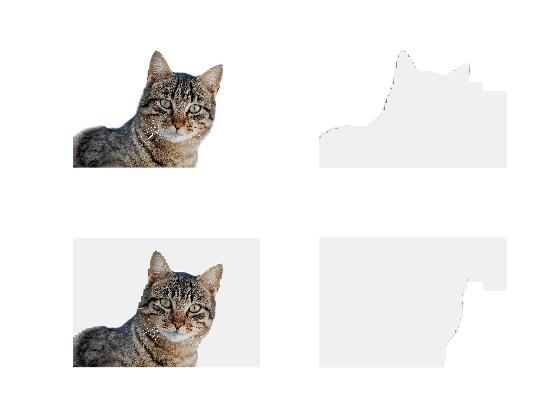
\includegraphics[width=.9\textwidth]{succ1.jpg}
	\caption{\texttt{cat\_march.jpg}, using HAC with $k = 3$, position + color features, feature normalization, and a resize factor of $0.025$.}
\end{figure}

\begin{figure}[H]
	\centering
	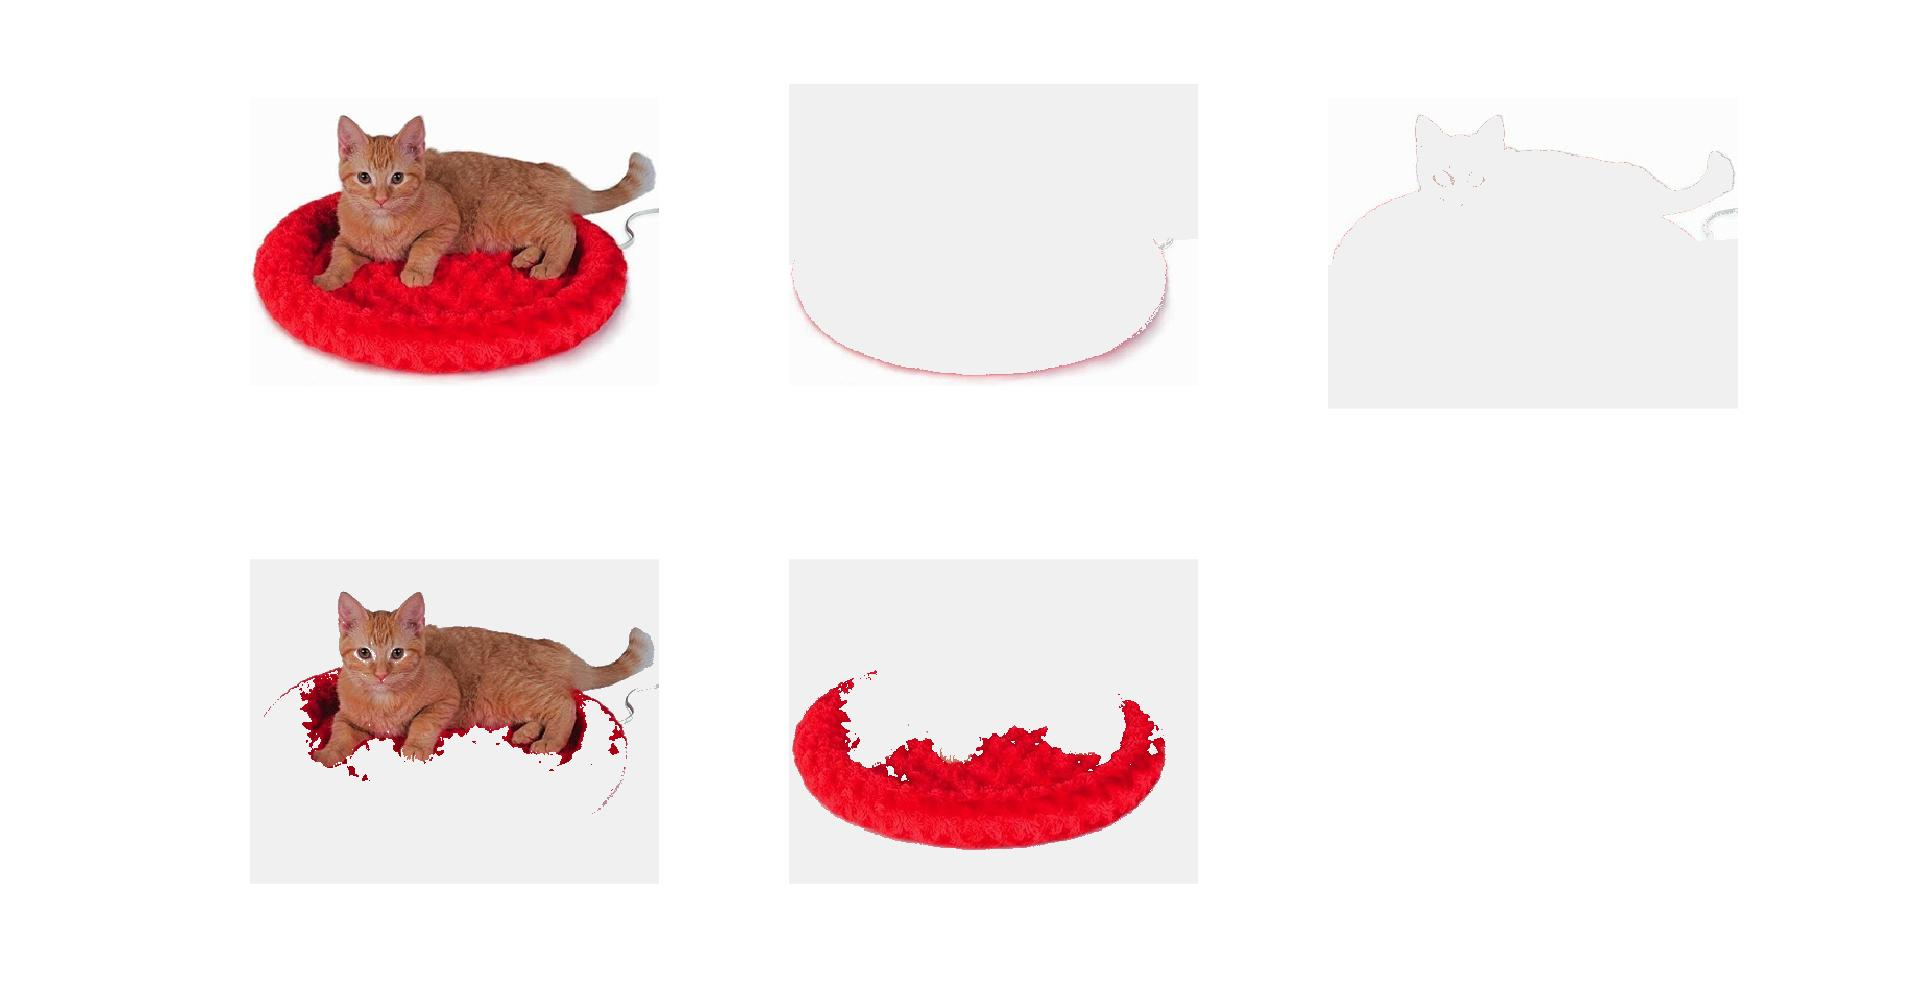
\includegraphics[width=.85\textwidth]{succ2.jpg}
	\caption{\texttt{Cat\_Bed.jpg}, using k-means clustering with $k = 4$, position + color features, and feature normalization.}
\end{figure}

\begin{figure}[H]
	\centering
	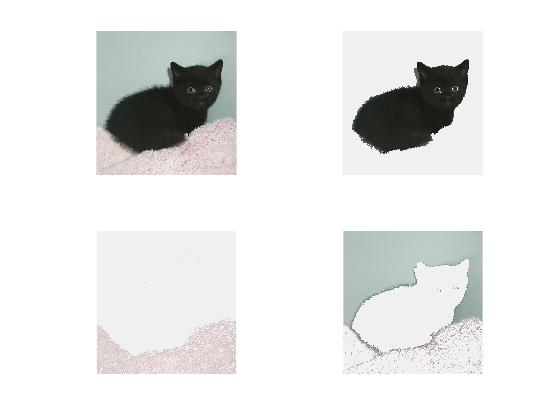
\includegraphics[width=.7\textwidth]{succ3.jpg}
	\caption{\texttt{black\_kitten\_star.jpg}, using k-means clustering with $k = 3$, color features, and no feature normalization.}
\end{figure}

\subsection{Unsuccessful Segmentations}
\begin{figure}[H]
	\centering
	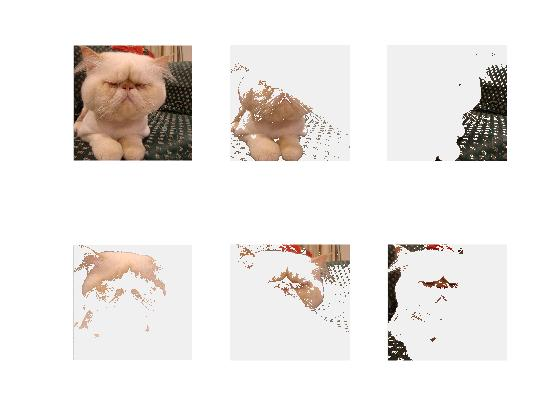
\includegraphics[width=.7\textwidth]{unsucc1.jpg}
	\caption{\texttt{cat\_grumpy.jpg}, using k-means clustering with $k = 5$, position + color features, and no feature normalization.}
\end{figure}

\begin{figure}[H]
	\centering
	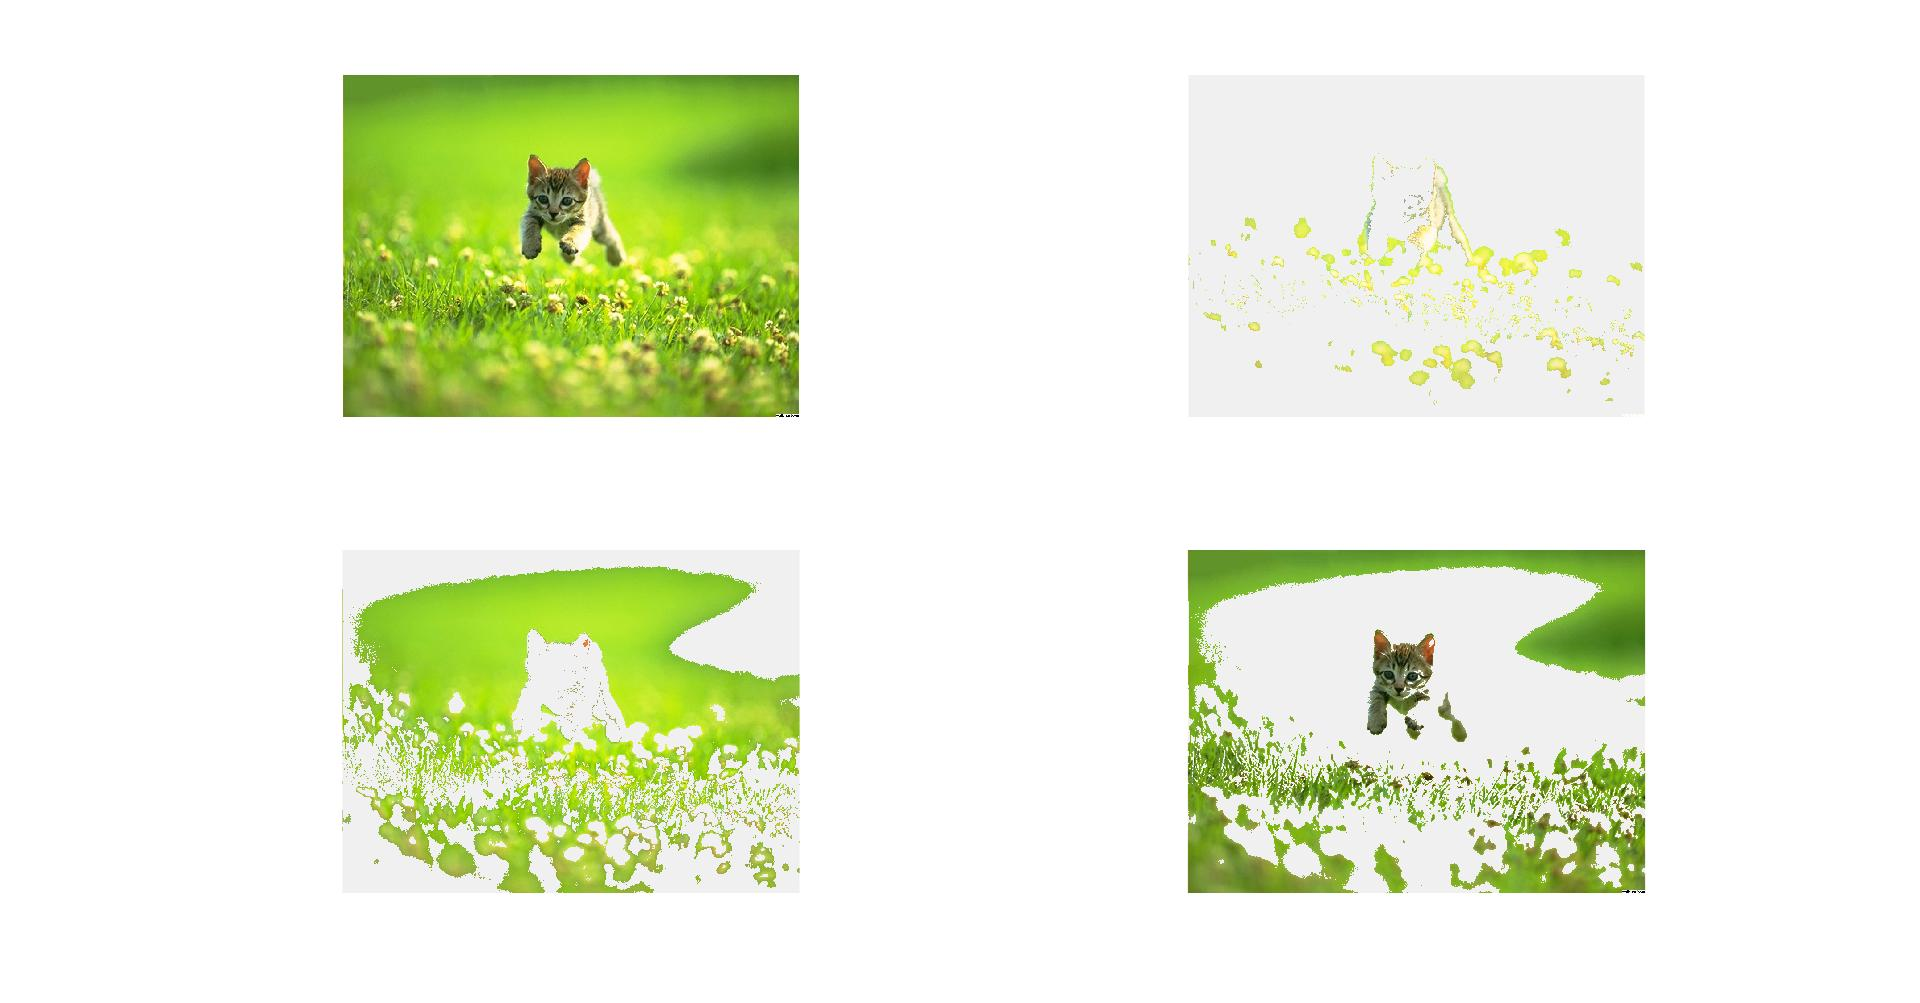
\includegraphics[width=.7\textwidth]{unsucc2.jpg}
	\caption{\texttt{cat-jumping-running-grass.jpg}, using k-means clustering with $k = 3$, color features, and feature normalization.}
\end{figure}

\begin{figure}[H]
	\centering
	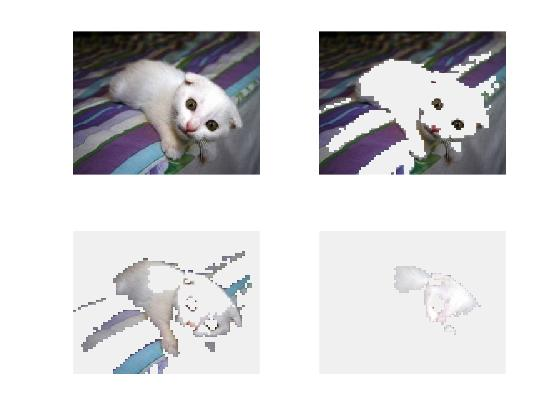
\includegraphics[width=.75\textwidth]{unsucc3.jpg}
	\caption{\texttt{kitten16.jpg}, using HAC with $k = 3$, color features, feature normalization, and a resize factor of $0.25$.}
\end{figure}

\subsection{Composite Images}
Using the script titled \texttt{GrabCat.m}, we were able to produce composite images by transferring segments from one image to another background image. This allowed us to create the two composite images shown below.

\begin{figure}[H]
	\centering
	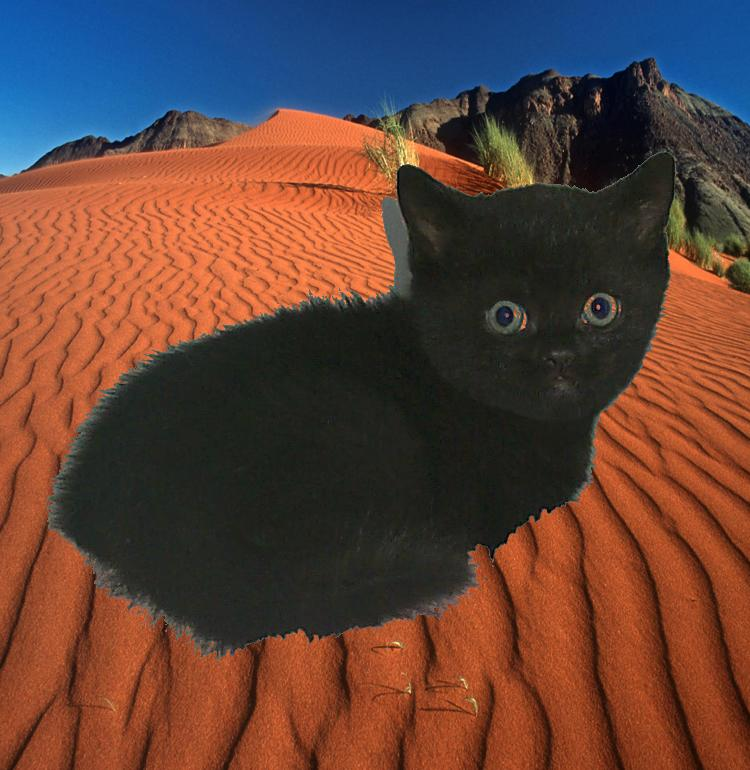
\includegraphics[width=.4\textwidth]{grabcat1.jpg}
	\caption{Input: \texttt{black\_kitten\_star.jpg, desert.jpg}, using k-means clustering with $k = 3$, color features, and feature normalization.}
\end{figure}

\begin{figure}[H]
	\centering
	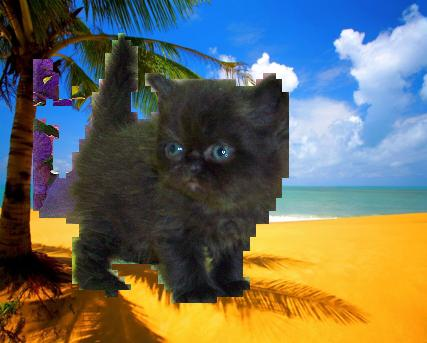
\includegraphics[width=.5\textwidth]{grabcat2.jpg}
	\caption{Input: \texttt{black\_kitten.jpg, beach.jpg}, using HAC with $k = 5$, color features, feature normalization, and a resize factor of $0.2$.}
\end{figure}

\section{Evaluation}
We evaluated in detail the effect of varying each of the segmentation parameters -- feature transform, feature normalization, clustering method, number of clusters, and the resize. Our results can be seen in the table below.

\begin{table}[H]
	\begin{adjustbox}{width=\columnwidth,center}
		\begin{tabular}{c c c c c c}
			\hline
			\textbf{Feature} & \textbf{Feature} & \textbf{Clustering} & \textbf{Number} & \textbf{Resize} & \textbf{Mean} \\
			\textbf{Transform} & \textbf{Normalization} & \textbf{Method} & \textbf{of Clusters} & \textbf{(Max Pixels)} & \textbf{Accuracy} \\
			\hline
			Color & Yes & K-Means & 3 & 50000 & .8341 \\
			Color & Yes & K-Means & 5 & 50000 & .8736 \\
			Color & Yes & K-Means & 7 & 50000 & .8795 \\
			Color & Yes & K-Means & 15 & 50000 & .9087 \\
			Color & Yes & K-Means & 30 & 50000 & .9228 \\
			Color & No  & K-Means & 5 & 50000 & .8680 \\
			Color/Position & Yes & K-Means & 5 & 50000 & .8765 \\
			Color/Position & No & K-Means & 5 & 50000 & .8802 \\
			Color/Edges & Yes & K-Means & 5 & 50000 & .7991\\
			Color/Edges & No & K-Means & 5 & 50000 & .8670 \\
			Color/Gradients & Yes & K-Means & 5 & 50000 & .7905 \\
			Color/Gradients & No & K-Means & 5 & 50000 & .8775 \\
			Color/Position/Edges & Yes & K-Means & 5 & 50000 & .7951 \\
			Color/Position/Edges & No & K-Means & 5 & 50000 & .8800 \\
			Color/Position/Edges/Gradients & Yes & K-Means & 5 & 50000 & .7924 \\
			Color/Position/Edges/Gradients & No & K-Means & 5 & 50000 & .8866 \\
			Color & Yes & HAC & 5 & 1000 & .8623 \\
			Color & Yes & HAC & 3 & 1000 & .8340 \\
			Color & Yes & HAC & 7 & 1000 & .8691 \\
			Color & Yes & HAC & 15 & 1000 & .8906 \\
			Color & Yes & HAC & 30 & 1000 & .9123 \\
			Color & No & HAC & 5 & 1000 & .8585 \\
			Color/Position & Yes & HAC & 5 & 1000 & .8531 \\
			Color/Position & No & HAC & 5 & 1000 & .8585 \\
			Color/Edges & Yes & HAC & 5 & 1000 & .9288 \\
			Color/Edges & No & HAC & 5 & 1000 & .8585 \\
			Color/Gradients & Yes & HAC & 5 & 1000 & .9108 \\
			Color/Gradients & No & HAC & 5 & 1000 & .8578 \\
			Color/Position/Edges & Yes & HAC & 5 & 1000 & .9256 \\
			Color/Position/Edges & No & HAC & 5 & 1000 & .8585 	\\
			Color/Position/Edges/Gradients & Yes & HAC & 5 & 1000 & .9052 \\
			Color/Position/Edges/Gradients & No & HAC & 5 & 1000 & .8550 \\
			Color & Yes & K-Means & 5 & 1000 & .8610 \\
			Color & Yes & K-Means & 5 & 10000 & .8649 \\
			Color & Yes & K-Means & 5 & 100000 & .8666 \\
			Color & Yes & HAC & 5 & 2000 & .8638 \\
			Color & Yes & HAC & 5 & 4000 & .8702 \\ \hline
		\end{tabular}
	\end{adjustbox}
	\caption{Mean Accuracy with varied Segmentation Parameters}
\end{table}

\textit{Note:} In order to better isolate the individual effects of varying the different segmentation parameters, we only tested the "most similar clusters" approach for the HAC algorithm. This would allow us to more thoroughly test the effect of other parameters on the quality of the segmentation.

\subsection{Qualitative Analysis}

\subsubsection{Effect of Segmentation Parameters}
Each of the segmentation parameters have various effects on the quality of the final segmentation:
\begin{itemize}
	\item \textit{Feature Transform} - 	The feature transform determines the qualities of points which should be considered as similar to be in a cluster. This could be color, position, gradients, or some combination of all of these. Depending on which transform is chosen, the overall quality of the segmentation can vary drastically.
	\item \textit{Feature Normalization} - When features in a transform are distributed in a vastly different way, it is likely that one feature will have a higher "weight" when finding the distance between clusters. With normalization, all the features are transformed to have the same mean and standard deviation, and will allow each feature in the transform to contribute equally in segmentation.
	\item \textit{Number of Clusters} - Generally, the number of clusters is a trade-off between accuracy and generalization. A higher number of clusters will be more accurate compared to the ground truth of a segmentation, especially when clusters can be chosen based on specific segments. But, as the number of clusters decreases, it is easier to have a more generalized view of the final segmentation.
	\item \textit{Clustering Method} - The clustering method will have varying effects on the final segmentation, depending on the data. A HAC segmentation can be better for when $k$ is not known, as it can simply stop when a good segmentation state is reached. Overall, the accuracy of these two methods are usually pretty similar, but HAC can also be much more accurate in certain situations despite taking a longer time to run.
	\item \textit{Resize} - A lower resize parameter will reduce the quality of the final segmentation. There will be fewer overall points to cluster, thus resulting in more blocky and less accurate segmentations.
\end{itemize}

\subsubsection{Effect of Parameters on Computation Speed}
For the k-means clustering algorithm, increasing the number of clusters drastically increases the runtime of the segmentation. This is because the k-means algorithm needs to do more comparisons on each point, as there are more possible centers that each point can be clustered into.


For the HAC algorithm, increasing the max pixels value slows the algorithm down to a crawl and requires much more RAM to compute the segmentation. Due to the nature of the algorithm, each pixel starts in its own cluster, and this requires a large amount of memory for images with many pixels. The max pixels also affects the k-mean runtime, but not as drastically as with HAC.

In both algorithms, normalization increases the runtime of the clustering, and this effect is more noticeable in feature transforms with many points (such as the \texttt{Color} / \texttt{Position} / \texttt{Edges} / \texttt{Gradients} transform). The choice of feature transform also affects runtime, as transforms with more data points cause the clustering to take longer to run. Also, feature transforms which require some external calculation (such as \texttt{Edges} or \texttt{Gradients}) affect computation speed, as it is computationally expensive to initially calculate these transforms.

\subsubsection{Image Properties}
	There are many properties of an image which can affect segmentation. Any amount of noise in an image will introduce difficulties to determine cluster distances, leading to inaccurate clusters. Also, an image which is busy, with lots of distinct objects or a complicated background, will be harder to segment. Finally, if the foreground and background of an image are visually similar, it may be hard to separate them into segments, as the cluster distance may be very close. 

\subsection{Quantitative Analysis}

Based on our quantitative analysis seen in the table above, we saw that each of the segmentation parameters affected the quality of the final foreground-background segmentation in different ways.

\begin{itemize}
	\item \textit{Feature Transform} - 
	\item \textit{Feature Normalization} -
	\item \textit{Number of Clusters} -
	\item \textit{Clustering Method} - 
	\item \textit{Resize} - 
\end{itemize}

In addition to the just the parameter-based effects, we also see that some images are simply more difficult to segment correctly than others. Inherently, images with a large and clear separation between the foreground and background are the easiest to separate (such as \texttt{cat\_march} or \texttt{Cat\_Bed}, as they are both subjects on a white background). Images with more complicated backgrounds are harder to segment (such as \texttt{kitten16}), and images in which the foreground and background are visually similar or blurred (such as \texttt{stripey-kitty}) also cause problems in the segmentation.

\subsection{Other Observations}
Another interesting thing we noticed in the behavior of these algorithms was in running the single-link Hierarchical Clustering algorithm. We noticed that, regardless of the feature transform, this algorithm would ultimately end up clustering nearly the entire image into one cluster. At a certain point, the foreground cluster would start "absorbing" the small background clusters, as the single-link distance would be the smallest between these clusters. This would be especially prevalent on some images such as \texttt{black\_kitten.jpg}, where we would need a $k = 300$ clusters for the foreground and background to be classified correctly.

\end{document}

